\section{The problem at hand}
We want to examine a hanging chain, with energy given as equation \eqref{Energi},
\begin{equation} \label{Energi}
E(x_{1,1},\cdots, x_{1,n},x_{2,1},\cdots,y_{2,n}):= \sum \limits^{n+1}_{i=1} m_i g \frac{x_{2,i}-x_{2,i-1}}{2}
\end{equation}
with constraints from equation \eqref{const}
\begin{equation} \label{const}
c_i(x_{1,1},\cdots, x_{1,n},x_{2,1},\cdots,x_{2,n}) = (x_{1,i}-x_{1,i-1})^2 + (x_{2,i}-x_{2,i-1})^2 - l^2_i = 0
\end{equation}
as a minimization problem, where $x_{1,i} $, $x_{2,i} $ are two spatial directions. We denote by $\Omega$ the set of feasible configurations of the chain, and $G_0 = (0,0)$, $G_1= (a,b)$ as the start and endpoint of the chain. We will first present some theoretical results, and then present a method to solve the problem.

\section{Some theory}
\subsection{Existence of solution}
First we want to show that there exists a solution. For that we get some help from theorem \ref{minim}.
\begin{theorem} \label{minim}
Assume that $f: \Omega \rightarrow \mathbb{R} \cup \{+\infty\}$. Then $f$ has at least one global minimizer in $\Omega$ if
\begin{itemize}
\item $\Omega$ is non-empty, closed and bounded.
\item $f: \Omega \rightarrow \mathbb{R}$ continuously.
\end{itemize}
\end{theorem}
The proof is omitted here, but the theorem can be further examined in \cite{thm1}.

\begin{proposition}
Equation \eqref{Energi} attains a minimum.
\end{proposition}
\begin{proof}
$\Omega$ is non-empty if and only if non of the numbers $||G_0-G_1||, l_1,\cdots,l_{n+1} $ are lagrer than the sum of all the others. Since equation (\ref{const}) is closed and bounded, so must $\Omega$ be. Clearly equation (\ref{Energi}) is linear, thus also continuous. 
%Continuous: $E$ is linear with $y_i$, and is therefore also countinuous.\\
%Bounded: Since $E$ is countiuous, and there is finitly many terms, and finite $y_i$'s, $\Omega$ must be bounded.\\
%Closed: Since the constraints contain is closure, so must $\Omega$.\\
\end{proof}

%% skrive det om så du bruker det som et teorem.
\subsection{KKT conditions}
KKT conditions are first order necessary conditions for a solution in nonlinear programming to be optimal \cite{KKT}. It is therefore of great importance that these conditions are fulfilled. The KKT conditions with equality constraints are given in definition \ref{KKT}.
%We adapt the notation $x = (x_1,\cdots x_n, y_1,\cdots,y_n)$.\\
%Assume $x^*$ is a optimal point, then the KKT-conditions, for a  minimization problem with only equality constraints are:

\begin{definition} \label{KKT} \cite{thm2}
Assume $x^*$ is an optimal point, and that
\[ \mathcal{L}(x^*;\lambda^*) = E(x^*)- \sum\limits_{i=1}^{n+1}\lambda_i c_i(x^*).\]
If the following conditions hold, we say that $x^*$ is a KKT point.

\begin{enumerate}
  %\centering
%\begin{itemize}
\item $\nabla_x \mathcal{L}(x^*,\lambda^*) = 0$
\item $c_i(x^*) = 0$
%\item $\lambda_i^* c_i = 0. $
%\end{itemize}
\end{enumerate}
\end{definition}


Substituting equation \eqref{Energi} and equation \eqref{const} into theorem \ref{KKT}, we obtain the KKT conditions for our problem, given in equation \eqref{KKT2}.
\begin{equation}\begin{aligned} \label{KKT2}
&\nabla_{x_{1,i}}\mathcal{L}(x^*,\lambda^*)&=& -2 \lambda_i (x_{1,i}-x_{1,i-1}) +2 \lambda_{i+1}(x_{1,i+1}-x_{1,i})&=0 \\
&\nabla_{x_{2,i}}\mathcal{L}(x^*,\lambda^*)&=& m_i g - 2 \lambda_i (x_{2,i}-x_{2,i-1}) +2 \lambda_{i+1}(x_{2,i+1}-x_{2,i})&=0 \\
&c_i(x) &=& (x_{1,i}-x_{1,i-1})^2 + (x_{2,i}-x_{2,i-1})^2-l^2_i&=0
\end{aligned}\end{equation}
We are also interested in what will happen if $a=0$, and there exists a feasible configuration of the chain where $x_{1,i} =0$ for all $i$. This means that the whole chain is contained in a vertical line. In this special case the conditions in equation \eqref{KKT2} simplifies a to equation \eqref{KKT3}.
\begin{equation}\begin{aligned}  \label{KKT3}
 m_i g - 2 \lambda_i (x_{2,i}-x_{2,i-1}) +2 \lambda_{i+1}(x_{2,i+1}-x_{2,i})&=0 \\
 (x_{2,i}-x_{2,i-1})^2-l^2_i&=0
\end{aligned}\end{equation}
More generally, equation \eqref{KKT3} can be written as equation \eqref{eqn:matcond}.
\begin{equation}\begin{aligned}\label{eqn:matcond}
\begin{pmatrix}
l_1 & -l_2 & 0& \cdots & 0 \\
0 & l_2 & -l_3 & \ddots & \vdots \\
\vdots & \ddots & \ddots & \ddots & 0 \\
0 & \cdots & 0 & l_n & -l_{n+1} \\
%0 & \cdots & \cdots & 0 & l_{n+1}
\end{pmatrix}
 \begin{pmatrix}
\lambda_1		\\
\lambda_2 	\\
\vdots 	\\ 
\lambda_n 		\\ 
\lambda_{n+1} 
\end{pmatrix}
= \frac{g}{2}
 \begin{pmatrix}
m_1		\\
m_2 		\\
\vdots 	\\ 
m_n 		\\ 
m_{n+1} 
\end{pmatrix}
\end{aligned}\end{equation}
The linear system presented in equation \eqref{eqn:matcond} has $n$ equations with $n+1$ unknowns and gives a solution. It is important to notice that even though the KKT conditions are satisfied, this might not be the optimal solution, some of the chains might be better off hanging to the side.

\subsection{LICQ conditions}
LICQ conditions with equality constraints are given in definition \ref{def:licq}. 
\begin{definition} \cite{LICQ} \label{def:licq}
Given a point $x$ and the set of all constraints, $C(x)$, we say that the linear independence constraint qualification (LICQ) holds if the set of constraint gradients $\{\nabla c_i(x), i \in C(x)\}$ is linearly independent.
\end{definition}
We now want to show that if the LICQ conditions does not hold, then all the links in the chain are parallel.
\begin{proof}
%We assume that all $\nabla_x c_i(x)$ are linearly dependant, and want to show that if this is the case, then all $\nabla c_i(x)$ must be paralell.
%For vectors to be paralell they must have the same incline number, that is 
%$ \nabla_x c_i(x) = \nabla c_l(x), \forall i \in{1,\cdots,n} $. 

Given two dependent vectors $a$, $b$, we know that there exists scalars $\lambda_1$ and $\lambda_2$ such that
\begin{align*}
\lambda_1 a+\lambda_2 b = 0  \rightarrow a = -\lambda_2/\lambda_1 b
\end{align*}
So they are parallel. By assumption, all $\nabla c_i(x)$ are linearly dependent thus all $ \nabla c_i(x)$ are parallel.
\end{proof}

\section{Solving the problem}
\subsection{How to find the solution} \label{sec:alg}
\begin{theorem}\cite{teoremet}
Let $x^*$ be a local solution at which LICQ is satisfied, $\lambda^*$ a Lagrange parameter such that the KKT-conditions hold and assume
\[\omega^\top \nabla_{xx}^2 \mathcal L(x^*,\lambda^*)\omega > 0,\,\forall \omega\neq 0.\]
Then the augmented Lagrangian method yields a solution.
\label{teoremet}\end{theorem}
\begin{proposition}
Equation \eqref{eqn:alm} has a minimum.
\end{proposition}
\begin{proof}
Note that the hessian of $\mathcal L(x^*,\lambda^*)$ is given by
\begin{equation*}
\begin{pmatrix}
 -2(\lambda_1 +\lambda_2) & 2\lambda_2 & 0 &  \\
2\lambda_1 & \ddots & \ddots & 0\\
 0 &  \ddots & \ddots  & 2\lambda_n \\
& 0& 2\lambda_{n} & -2(\lambda_n +\lambda_{n+1})
\end{pmatrix}
\end{equation*}

By Gerschgorin's theorem \cite{gresgorian}, this matrix is positive definite when $\lambda_i < 0, \forall i$, which must be assumed. Thus the conditions of theorem \ref{teoremet} is satisfied, so the augmented Lagrangian has a solution. In other words, there exists a minimum. 
\end{proof}

The greatest difficulty with the problem presented in equation \eqref{Energi}  is the need to satisfy constraints in equation \eqref{const}. The augmented Lagrangian method is a method that simplifies the problem to only minimize equation \eqref{eqn:alm} in each iteration for suitable $\lambda,\,\mu$. The full method is given in algorithm \ref{alg:alm}.
\begin{align} \label{eqn:alm}
\mathcal{L}(x,\lambda,\mu) = E(x) - \sum \limits_{i = 1}^{n+1} \lambda c_i(x) + \frac{\mu}{2} \sum \limits_{i =1}^{n+1}c_i(x) 
\end{align}
Algorithm \ref{alg:back} is the minimizer used in algorithm \ref{alg:alm} to minimize equation \eqref{eqn:alm}. When choosing a minimizer, there are two different choices, line search, and trust region methods. We use a line search method called Newton's method, which uses steepest decent method when Newtons method does not give a decent direction. The minimizer also uses a backtracking algorithm for choosing the step length. The dogleg method was also implemented, but did not give a suitable answer, the reason for this is unknown.

\begin{algorithm} 
\begin{algorithmic} \caption{\cite{ALM}Augmented lagrangian metod} \label{alg:alm} 
\STATE Start with $x_0$, $\lambda_0$ and $\mu_0$
\FOR{$k = 1,2,\cdots$} 
   \STATE Find $x_{k+1}$ mimimizing $\mathcal{L}(x_k,\lambda^k_i,\mu_k)$
   \STATE Set $\lambda_i^{k+1} = \lambda^k_i-\mu_kc_i(x_{k+1})$
    \STATE Choose $ \mu_{k+1} > \mu_k$
\ENDFOR
\end{algorithmic} 
\end{algorithm}


\begin{algorithm}  %\cite{backtracking} %\cite{newton}
\begin{algorithmic} \caption{\cite{backtracking}Newton's method and steepest decent method with backtracking} \label{alg:back}
\STATE Start with $x_0$, $\lambda_0$ and $\mu_0$
\STATE Set $\gamma < 1$, $\rho < 1$
\FOR{$k = 1,2,\cdots$} 
   \STATE Find $\mathcal{N} = \nabla C(x_k)$, $\mathcal{H} = \nabla^2C(x_k)$.
   \STATE Set $p = -\mathcal{H} \backslash \mathcal{N}$
   	\IF{$\mathcal{N}^{\top}\mathcal{H}\mathcal{N} \geq 0$}
   	\STATE Set $p = -\mathcal{N}$
   	\ENDIF
    \STATE Set $\alpha = 1$
    \WHILE{$E(x_k+\alpha p) > E(x_k) + \gamma \alpha \mathcal{N}'p $}
    \STATE $\alpha = \rho \alpha $
    \ENDWHILE
    \STATE $x_{k+1} = x_{k} + \alpha p$
\ENDFOR
\end{algorithmic} 
\end{algorithm}


%!!!!!!!!!!!!!Harald må vise at metoden vil gi rett løsning!!!!!!!!!!!!!!!!!!!!!!
\subsection{Implementation}
The algorithms presented in section \ref{sec:alg} where implemented, and can be run with the script \texttt{runthing.m}, which should be self explanatory. The implementation of algorithm \ref{alg:alm} is called \texttt{alf.m}, and the implementation of algorithm \ref{alg:back} is called \texttt{minimizer.m}. 

\section{Some results}
Some results from running \texttt{runthing.m} with different chains are shown in figure \ref{fig:exp}. 

\begin{figure}
        \centering
        \begin{subfigure}[b]{0.45\textwidth}
                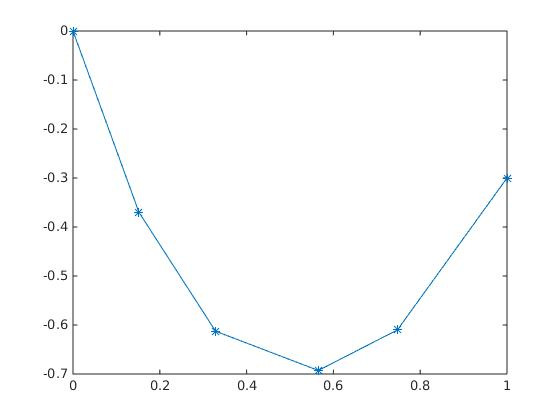
\includegraphics[width=\textwidth]{test1.jpg}
                \caption{$l,m = [0.4,0.3,0.25,0.2,0.4]$ with endpoint $G_1 = (1,-0.3)$. }
                \label{fig:test1}
        \end{subfigure}%
        ~
        \begin{subfigure}[b]{0.45\textwidth}
                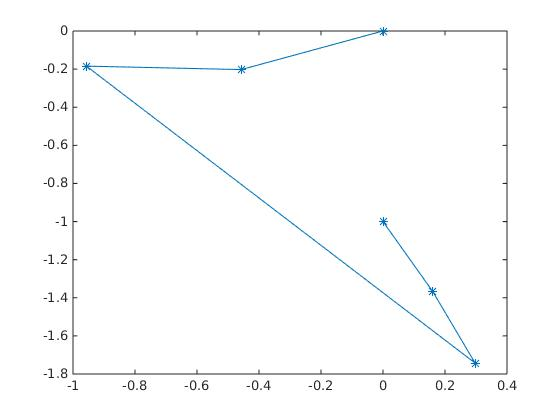
\includegraphics[width=\textwidth]{test2.jpg}
                \caption{$l,m = [0.5,0.5,2,0.4,0.4]$ with endpoint $G_1 = (0,-1)$. }
                \label{fig:test2}
        \end{subfigure}
        
        \begin{subfigure}[b]{0.45\textwidth}
                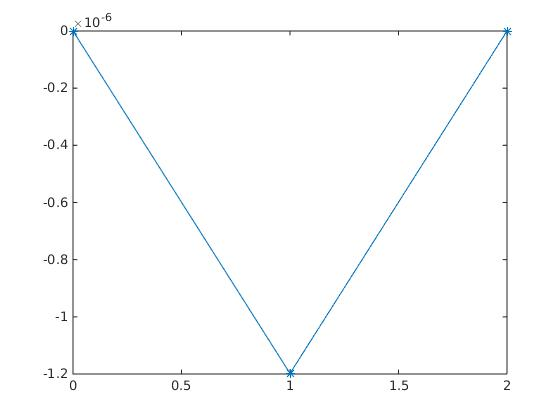
\includegraphics[width=\textwidth]{test3.jpg}
                \caption{$l,m = [1,1]$ with endpoint $G_1 = (2,0)$.}
                \label{fig:test3}
        \end{subfigure}
        ~
        \begin{subfigure}[b]{0.45\textwidth}
                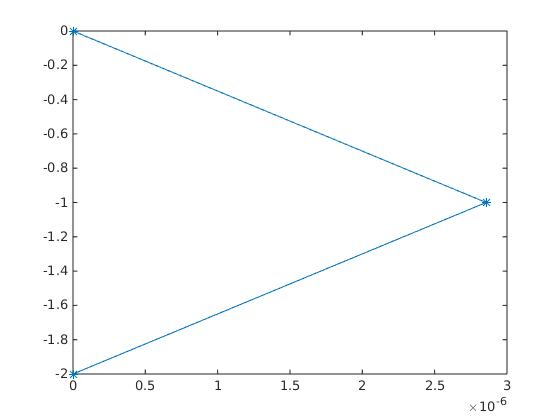
\includegraphics[width=\textwidth]{test4.jpg}
                \caption{$l,m = [1,1]$ with endpoint $G_1 = (0,-2)$.}
                \label{fig:test4}
        \end{subfigure}
        \caption{Examples of hanging chains}\label{fig:exp}
\end{figure}
\subsection{What about run time?}
Due to the random initial guess for $x_0$, run time is quite arbitrary, and we did not find any clear relation between number of chain links and the time it takes to find a solution. The reason for the random initial guess at $x_0$, are manifold. First, a random guess is not sure to be any worse, or better, than a deterministic. Second if it does not work the first try, there is a chance that it might work the second try. Third, there might be different solutions, a deterministic initial guess would only find one, while a random guess might find more (if run multiple times). The clear downside to this is the run time. As an indication of how long it takes, some approximate estimates are presented in table \ref{tab:time}.
\begin{table}[]
\centering
\begin{tabular}{l l}
Number of chains & time elapsed in seconds \\
\hline
5 &  $\sim 0.2-0.5$\\
10 & $\sim 5-10 $ \\
15 & $\sim 6-900$ \\
\end{tabular}
\caption{Run time for different problem sizes}
\label{tab:time}
\end{table}

\section{Discussion}
\texttt{runthing.m} gives the correct answer, but does so very slowly. 